\documentclass[docmute]{article}
\documentclass{article} % Use the article document class

% AMS packages for enhanced math typesetting and symbols:
\usepackage{amsmath}  % Provides enhanced math features like align, gather, etc.
\usepackage{amssymb}  % Provides additional math symbols
\usepackage{amsthm}   % Enables theorem-like environments

% Package for customizing list environments:
\usepackage{enumitem} % Allows control over layout of lists (itemize, enumerate, etc.)

% Full-page layout package:
\usepackage{fullpage} % Uses more of the page area by reducing margins

% TikZ package for drawing graphics:
\usepackage{tikz}     % Used for creating high-quality diagrams and figures

% Microtype package for typographical enhancements:
\usepackage{microtype} % Improves justification, kerning, and overall appearance

% Package for typesetting polynomials:
\usepackage{polynom}  % Provides commands for polynomial long division and related tasks

% Package for controlling figure placement:
\usepackage{placeins} % Provides the \FloatBarrier command to control floating environments

% Forest package for drawing trees:
\usepackage{forest}   % Simplifies the creation of tree diagrams

% Package to allow one LaTeX file to input another:
\usepackage{docmute}  % Allows this file to be included in another document without reloading the preamble

% Load additional TikZ libraries:
\usetikzlibrary{trees} % Provides additional tree-specific commands for TikZ

% Define theorem-like environments using amsthm:
\newtheorem{corollary}{Corollary} % Defines a new "corollary" environment
\newtheorem{lemma}{Lemma}         % Defines a new "lemma" environment


\title{Generating Functions}
\author{Tomasz Brengos \\  
Committers : Mykhailo Moroz, Mihail Orlov}
\date{}

\begin{document}
\maketitle
\section{Generating Series}

Instead of viewing a sequence as a function that returns its \(n\)th term, a \emph{generating series} packages all of its terms into a single power series whose coefficients are exactly the sequence entries.  Concretely, the sequence
\[
2,\;3,\;5,\;8,\;12,\;\dots
\]
is encoded by the generating series
\[
2 + 3x + 5x^2 + 8x^3 + 12x^4 + \cdots.
\]

In general, given any sequence \(\{c_n\}_{n\ge0}\), its generating series is the formal power series

\[
G(x) \;=\; \sum_{n=0}^\infty c_n x^n 
\;=\;
c_0 + c_1 x + c_2 x^2 + c_3 x^3 + \cdots.
\]

We say that \(G(x)\) “generates” the sequence \(\{c_n\}\) because each coefficient of \(x^n\) in \(G(x)\) is precisely \(c_n\).  Generating series turn sequence‑based problems into algebraic manipulations of power series, a technique we will exploit heavily in what follows.

\subsection*{Recall of the Basic Series}
\paragraph{A Geometric View of the Binary Series}
\begin{figure}[ht]
  \centering
  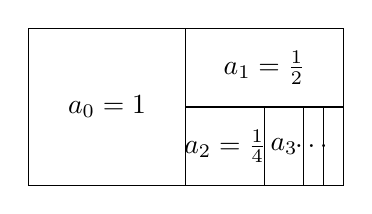
\begin{tikzpicture}[scale=2]
      % Draw outer rectangle (width=2, height=1)
      \draw (0,0) rectangle (2,1);
  
      % Partition line between a0 and the rest
      \draw (1,0) -- (1,1);
  
      % Label a0
      \node at (0.5,0.5) {$a_0 = 1$};
  
      % Horizontal partition for the right half (top sub-rectangle a1)
      \draw (1,0.5) -- (2,0.5);
      \node at (1.5,0.75) {$a_1 = \frac{1}{2}$};
  
      % Vertical partition for the bottom half (a2, a3, ...)
      \draw (1.5,0) -- (1.5,0.5);
      \node at (1.25,0.25) {$a_2 = \frac{1}{4}$};
  
      % Subdivide further for illustration (a3, a4, …)
      \draw (1.75,0) -- (1.75,0.5);
      \draw (1.875,0) -- (1.875,0.5);
  
      % Place a3 label (you can add more if you like)
      \node at (1.625,0.25) {$a_3$};
      \node at (1.8125,0.25) {$\dots$};
\end{tikzpicture}
\caption{A geometric interpretation of the binary series, showing how 
\(\sum_{n=0}^{\infty} \tfrac{1}{2^n} = 2\).}
\end{figure}
For \(|x| < 1\), we have the infinite geometric series
\[
\frac{1}{1-x} = 1 + x + x^2 + x^3 + \cdots = \sum_{n=0}^{\infty} x^n.
\]
We now present a quick proof of this result by performing long division of \(1\) by \(1-x\).

\[
\renewcommand{\arraystretch}{1.3}
\begin{array}{r|l}
 & 1 + x + x^2 + x^3 + \cdots \\ % quotient
1 - x & 1  \\ % divisor | dividend
\hline
 & \underline{1 - x} \\
 & x \\
 & \underline{x - x^2} \\
 & x^2 \\
 & \underline{x^2 - x^3} \\
 & x^3 \\
 & \vdots
\end{array}
\]


The process works as follows:
The long‑division proceeds by repeatedly dividing the current remainder by the leading term of the divisor, producing one new power of \(x\) at each step:

\begin{enumerate}
  \item Divide \(1\) by \(1-x\). The multiplier needed to eliminate the constant term is \(1\), so 
  \[
    1 - 1\cdot(1-x) = x.
  \]
  Thus the first summand is \(1\), leaving a remainder of \(x\).

  \item Divide the remainder \(x\) by \(1-x\). The multiplier is \(x\), so
  \[
    x - x\cdot(1-x) = x^2.
  \]
  Hence the second summand is \(x\), leaving a remainder of \(x^2\).

  \item Divide \(x^2\) by \(1-x\). The multiplier is \(x^2\), giving
  \[
    x^2 - x^2\cdot(1-x) = x^3.
  \]
  Therefore the third summand is \(x^2\), with remainder \(x^3\).

  \item Continuing in this fashion produces the infinite series
  \[
    \frac{1}{1-x} = 1 + x + x^2 + x^3 + \cdots.
  \]
\end{enumerate}


Continuing indefinitely produces
\[
\frac{1}{1-x} = 1 + x + x^2 + x^3 + \cdots = \sum_{n=0}^\infty x^n,
\]
as claimed. \par
\noindent We will use this fact in further examples throughout the notes.

\section{Building Generating Functions}

The simplest (or “basic”) generating function is
\[
\frac{1}{1-x} = 1 + x + x^2 + x^3 + \cdots,
\]
which generates the constant sequence \(1,1,1,\dots\).

\medskip
\noindent
\textbf{Replacing \(x\) with \(-x\):}
\[
\frac{1}{1-(-x)} = \frac{1}{1+x} = 1 - x + x^2 - x^3 + \cdots,
\]
generating \(1,-1,1,-1,\dots\).

\medskip
\noindent
\textbf{Replacing \(x\) with \(3x\):}
\[
\frac{1}{1-3x} = 1 + 3x + 9x^2 + 27x^3 + \cdots,
\]
generating \(1,3,9,27,\dots\).

\medskip
\noindent
\textbf{Scaling a sequence by 3:}
\[
\frac{3}{1-3x} = 3 + 9x + 27x^2 + 81x^3 + \cdots,
\]
generating \(3,9,27,81,\dots\).

\medskip
\noindent
\textbf{Termwise addition of sequences:}\\
Adding the generating functions for \(1,1,1,\dots\) and \(1,3,9,\dots\) gives
\[
\frac{1}{1-x} + \frac{1}{1-3x}
= 2 + 4x + 10x^2 + 28x^3 + \cdots,
\]
which generates \(2,4,10,28,\dots\).

\medskip
\noindent
\textbf{Replacing \(x\) with \(x^2\):}
\[
\frac{1}{1-x^2} = 1 + x^2 + x^4 + x^6 + \cdots,
\]
generating \(1,0,1,0,1,0,\dots\).

\medskip
\noindent
\textbf{Shifting a sequence:}\\
Multiplying by \(x\) shifts all coefficients right by one:
\[
\frac{x}{1-3x} = 0 + x + 3x^2 + 9x^3 + \cdots,
\]
generating \(0,1,3,9,\dots\), and
\[
\frac{x}{1-x^2} = 0 + x + 0x^2 + x^3 + \cdots,
\]
generating \(0,1,0,1,\dots\).

\medskip
\noindent
\textbf{Combining shifted sequences:}\\
Adding the two “even‑odd” generating functions recovers
\[
\frac{1}{1-x^2} + \frac{x}{1-x^2} = \frac{1+x}{1-x^2} = \frac{1}{1-x},
\]
which generates \(1,1,1,1,\dots\).

\medskip
\noindent
\textbf{Differentiation:}\\
Differentiating the basic Generating Function
\[
\frac{d}{dx}\!\Bigl(\frac{1}{1-x}\Bigr)
= \frac{1}{(1-x)^2}
= 1 + 2x + 3x^2 + 4x^3 + \cdots,
\]
yields the generating function for \(1,2,3,4,\dots\).


\medskip

\FloatBarrier            % ensure the Differentiation figure/text finishes here

\section{Recurrence Relations \& Generating Functions}

We conclude with an example of one of the many reasons studying generating functions is helpful: solving recurrence relations via algebraic manipulation of power series.

\paragraph{Example: Tower of Hanoi}  
The minimum number of moves required to transfer \(n\) disks satisfies
\[
a_0 = 0,\quad
a_1 = 1,\quad
a_n = 2\,a_{n-1} + 1 \quad(n\ge1),
\]
giving the sequence
\[
0,\;1,\;3,\;7,\;15,\;31,\dots
\]

\begin{figure}[ht]
  \centering
  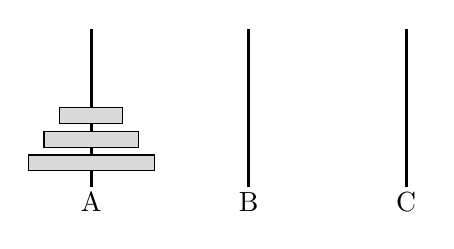
\begin{tikzpicture}[scale=1]
    % Draw three pegs
    \foreach \x in {0,2,4} {
      \draw[line width=1pt] (\x,0) -- (\x,2);
    }
    % Draw disks on left peg
    \foreach \i/\w in {0.2/1.6,0.5/1.2,0.8/0.8} {
      \draw[fill=gray!30] (0-\w/2,\i) rectangle (0+\w/2,\i+0.2);
    }
    \node at (0,-0.2) {A};
    \node at (2,-0.2) {B};
    \node at (4,-0.2) {C};
  \end{tikzpicture}
  \caption{Initial configuration for Tower of Hanoi (3 disks).}
\end{figure}

Define the generating function
\[
f(x) = \sum_{n=0}^\infty a_n x^n.
\]
Using the recurrence for \(n\ge1\):
\[
\sum_{n=1}^\infty a_n x^n 
= \sum_{n=1}^\infty \bigl(2a_{n-1}+1\bigr)x^n
= 2x\sum_{n=0}^\infty a_n x^n + \sum_{n=1}^\infty x^n,
\]
so
\[
f(x) - a_0 = 2x\,f(x) + \frac{x}{1-x},
\]
and since \(a_0=0\),
\[
f(x) = \frac{x}{(1-x)(1-2x)}.
\]

Performing partial fractions:
\[
\frac{x}{(1-x)(1-2x)}
= \frac{-1}{1-x} + \frac{1}{1-2x},
\]
hence
\[
f(x) = -\frac{1}{1-x} + \frac{1}{1-2x}.
\]

Extracting coefficients yields the closed‑form solution
\[
a_n = 2^n - 1,
\]
confirming the well‑known formula for the Tower of Hanoi moves.
\FloatBarrier

\section{Introduction to the Fibonacci Sequence}
The Fibonacci sequence famously arises from a puzzle involving rabbit populations.
Imagine starting with a single pair of rabbits that takes one month to mature.
After maturing, each pair produces a new pair of rabbits every month.
Mathematically, if \(F_n\) represents the number of rabbit pairs in month \(n\),
the sequence satisfies the initial conditions
\[
F_0 = 0, \quad F_1 = 1,
\]
and the recurrence
\[
F_{n+2} = F_{n+1} + F_n \quad \text{for} \; n \ge 0.
\]

\begin{figure}[ht]
  \centering
  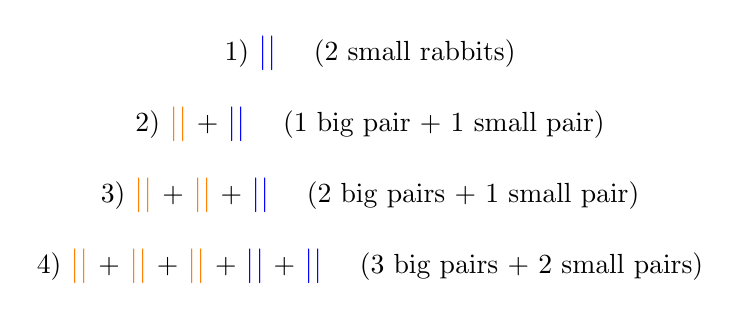
\begin{tikzpicture}[x=1cm, y=0.9cm]
      % Month 1
      \node at (0,0) {1) \(\textcolor{blue}{\big|\big|}\) \quad (2 small rabbits)};
      % Month 2
      \node at (0,-1) {2) \(\textcolor{orange}{\big|\big|}\) + \(\textcolor{blue}{\big|\big|}\) 
        \quad (1 big pair + 1 small pair)};
      % Month 3
      \node at (0,-2) {3) \(\textcolor{orange}{\big|\big|}\) + \(\textcolor{orange}{\big|\big|}\) + \(\textcolor{blue}{\big|\big|}\)
        \quad (2 big pairs + 1 small pair)};
      % Month 4
      \node at (0,-3) {4) \(\textcolor{orange}{\big|\big|}\) + \(\textcolor{orange}{\big|\big|}\) + \(\textcolor{orange}{\big|\big|}\) 
        + \(\textcolor{blue}{\big|\big|}\) + \(\textcolor{blue}{\big|\big|}\)
        \quad (3 big pairs + 2 small pairs)};
\end{tikzpicture}
\caption{Illustration of rabbit pairs over successive months. 
Blue bars represent small rabbits; orange bars represent big (mature) rabbits.}
\end{figure}

Q: is there a non-recursive (closed-form) formula for \(F_n\) ?
\paragraph{Idea: consider and calculate it}

\section{Deriving the Closed-Form for the Fibonacci Sequence}

\paragraph{Step 1: Define the generating function.}
Let \(\{F_n\}_{n=0}^{\infty}\) be the Fibonacci sequence with 
\[
F_0 = 0, \quad F_1 = 1, \quad F_{n+2} = F_{n+1} + F_n \quad (n \ge 0).
\]
Define the generating function
\[
f(x) \;=\; \sum_{n=0}^{\infty} F_n\,x^n.
\]
We aim to find a closed-form expression for \(f(x)\), and then extract a formula for \(F_n\).

\paragraph{Step 2: Use the Fibonacci recurrence in \(f(x)\).}
Starting from
\[
f(x) \;=\; F_0 + F_1 x + \sum_{n=2}^{\infty} F_n\,x^n,
\]
and noting \(F_0=0\), \(F_1=1\), we have
\[
f(x) \;=\; x + \sum_{n=2}^{\infty} \bigl(F_{n-1} + F_{n-2}\bigr)\,x^n
\]
because \(F_n = F_{n-1} + F_{n-2}\) for \(n\ge2\). Separate the sums:
\[
f(x)
= x
+ \sum_{n=2}^{\infty} F_{n-1}\,x^n
+ \sum_{n=2}^{\infty} F_{n-2}\,x^n.
\]
Shift indices to factor out \(f(x)\):
\[
\sum_{n=2}^{\infty} F_{n-1}\,x^n 
= x \sum_{n=2}^{\infty} F_{n-1}\,x^{n-1} 
= x \sum_{m=1}^{\infty} F_m\,x^m 
= x \bigl(f(x) - F_0\bigr) 
= x\,f(x),
\]
since \(F_0=0\). Similarly,
\[
\sum_{n=2}^{\infty} F_{n-2}\,x^n 
= x^2 \sum_{n=2}^{\infty} F_{n-2}\,x^{n-2}
= x^2 \sum_{k=0}^{\infty} F_k\,x^k
= x^2\,f(x).
\]
Hence,
\[
f(x) = x + x\,f(x) + x^2\,f(x) 
\;\;\Longrightarrow\;\;
f(x)\bigl(1 - x - x^2\bigr) = x.
\]
Thus,
\[
f(x) = \frac{x}{\,1 - x - x^2\,}.
\]

\paragraph{Step 3: Partial-Fraction Decomposition (as in the images).}

First, rewrite
\[
\frac{1}{1 - x - x^2}
\;=\;
\frac{1}{-\bigl(x^2 + x - 1\bigr)}
\;=\;
-\,\frac{1}{x^2 + x - 1}.
\]

\noindent
Next, factor \(x^2 + x - 1\). Observe that the roots of
\[
x^2 + x - 1 \;=\; 0
\]
are
\[
x \;=\; -\,\frac{1 + \sqrt{5}}{2}
\quad\text{and}\quad
x \;=\; -\,\frac{1 - \sqrt{5}}{2}.
\]
Hence,
\[
x^2 + x - 1
\;=\;
\Bigl(x + \tfrac{1 + \sqrt{5}}{2}\Bigr)
\;\cdot\;
\Bigl(x + \tfrac{1 - \sqrt{5}}{2}\Bigr).
\]
Therefore,
\[
-\,\frac{1}{x^2 + x - 1}
\;=\;
-\,\frac{1}{\Bigl(x + \tfrac{1 + \sqrt{5}}{2}\Bigr)\,\Bigl(x + \tfrac{1 - \sqrt{5}}{2}\Bigr)}.
\]
We look for constants \(A\) and \(B\) such that
\[
-\,\frac{1}{\Bigl(x + \tfrac{1 + \sqrt{5}}{2}\Bigr)\,\Bigl(x + \tfrac{1 - \sqrt{5}}{2}\Bigr)}
\;=\;
\frac{A}{\,x + \tfrac{1 + \sqrt{5}}{2}\,}
\;+\;
\frac{B}{\,x + \tfrac{1 - \sqrt{5}}{2}\,}.
\]


\paragraph{Step 4: Solve for \(A\) and \(B\).}

Comparing coefficients of \(x\) and the constant term in
\[
-\,1
\;=\;
A\Bigl(x + \beta\Bigr)
\;+\;
B\Bigl(x + \alpha\Bigr),
\]
we obtain the system
\[
\begin{cases}
A + B = 0, \\[4pt]
A\,\beta + B\,\alpha = -\,1.
\end{cases}
\]
It follows that
\[
B = -\,A,
\quad
A\,(\beta - \alpha) = -\,1
\;\;\Longrightarrow\;\;
A = \frac{1}{\alpha - \beta}
\quad\text{and}\quad
B = -\,\frac{1}{\alpha - \beta}.
\]
Hence,
\[
-\,\frac{1}{(x+\alpha)(x+\beta)}
\;=\;
\frac{1}{\alpha - \beta}\,\frac{1}{\,x+\alpha\,}
\;-\;
\frac{1}{\alpha - \beta}\,\frac{1}{\,x+\beta\,}.
\]

\paragraph{Step 5: Combine with the earlier factor \(-1\) and rewrite.}

Recalling that
\[
\frac{1}{1 - x - x^2}
\;=\;
-\,\frac{1}{\,x^2 + x - 1\,}
\;=\;
-\,\frac{1}{\,(x+\alpha)\,(x+\beta)\,},
\]
we combine the above result to conclude
\[
\frac{1}{1 - x - x^2}
\;=\;
\frac{1}{\alpha - \beta}
\left(
\frac{1}{\,x+\alpha\,}
\;-\;
\frac{1}{\,x+\beta\,}
\right).
\]

\paragraph{Step 6: Expand each term in a power series.}

Notice that
\[
\frac{1}{x + \alpha}
\;=\;
\frac{1}{\alpha}\,\frac{1}{1 + \tfrac{x}{\alpha}}
\;=\;
\frac{1}{\alpha}\,\sum_{n=0}^\infty \bigl(-\tfrac{x}{\alpha}\bigr)^{n}
\;=\;
\sum_{n=0}^\infty
\frac{(-1)^n}{\,\alpha^{\,n+1}\!}\,
x^n,
\]
valid for \(\bigl|\tfrac{x}{\alpha}\bigr| < 1\).  Similarly,
\[
\frac{1}{x + \beta}
\;=\;
\sum_{n=0}^\infty
\frac{(-1)^n}{\,\beta^{\,n+1}\!}\,
x^n.
\]
Hence,
\[
\frac{1}{1 - x - x^2}
\;=\;
\frac{1}{\alpha - \beta}
\left[
\sum_{n=0}^\infty \frac{(-1)^n}{\,\alpha^{\,n+1}\!}\,x^n
\;-\;
\sum_{n=0}^\infty \frac{(-1)^n}{\,\beta^{\,n+1}\!}\,x^n
\right]
=
\sum_{n=0}^\infty
\left[
\frac{1}{\alpha - \beta}
\Bigl(
\frac{(-1)^n}{\,\alpha^{\,n+1}\!}
\;-\;
\frac{(-1)^n}{\,\beta^{\,n+1}\!}
\Bigr)
\right]
x^n.
\]

\paragraph{Step 7: Identify Fibonacci numbers.}

Recall that \(\alpha - \beta = \sqrt{5}\), and
\[
F_n
\;=\;
\frac{\alpha^n - \beta^n}{\,\alpha - \beta\,}
\;=\;
\frac{\alpha^n - \beta^n}{\,\sqrt{5}\,}.
\]
One checks (or uses known identities) to see that the coefficient of \(x^n\) in the above power series is exactly \(F_n\).  Consequently,
\[
\sum_{n=0}^\infty F_n \, x^n
\;=\;
\frac{1}{\,1 - x - x^2\,},
\]
which is the generating function for the Fibonacci sequence.

\paragraph{Conclusion.}
We have shown that the generating function for the Fibonacci sequence is 
\(\tfrac{x}{1 - x - x^2}\).  
Through partial fractions and comparing coefficients, we deduced that
\[
F_n = \frac{\alpha^n - \beta^n}{\sqrt{5}}.
\]
This gives a non-recursive (closed-form) expression for \(F_n\), completing the derivation.

\section{More examples}

In earlier sections (see, e.g., \emph{A Geometric View of the Binary Series} on page~14), we explored methods to solve recurrences and introduced generating functions as a tool to transform sequences into functions. In this section, we briefly reiterate these ideas and demonstrate, through several examples, how generating functions serve as a bridge between discrete mathematics and calculus.

\paragraph{Example 1: Constant Sequence.}  
Consider the sequence defined by
\[
a_n=1 \quad \text{for all } n\ge0,
\]
so that the sequence is
\[
1,\,1,\,1,\dots.
\]
By the geometric series formula (proved earlier), its generating function is given by
\[
f(x)=\sum_{n=0}^{\infty} x^n=\frac{1}{1-x}, \quad |x|<1.
\]

\paragraph{Example 2: Exponential Sequence.}  
Now, let
\[
a_n=\frac{1}{n!}.
\]
Then the generating function is
\[
f(x)=\sum_{n=0}^{\infty} \frac{x^n}{n!}=e^x, \quad x\in\mathbb{R}.
\]
A partial justification of this result can be obtained by recalling the Taylor series expansion of the exponential function. Although a complete treatment of Taylor series is a topic in calculus (not yet covered in this course), note that differentiating the power series term-by-term confirms the identity.

\paragraph{Example 3: Binomial Coefficient Sequence.}  
Consider the sequence defined by
\[
a_n=\binom{n+k}{k}.
\]
\textbf{Theorem.} The generating function for this sequence is
\[
f(x)=\sum_{n=0}^{\infty}\binom{n+k}{k}x^n=\frac{1}{(1-x)^{k+1}}, \quad |x|<1.
\]
\newpage
\textit{Proof.}  
\begin{itemize}
    \item For \(k=1\): Note that
    \[
    \ a_n = \binom{n+1}{1} = n+1,
    \]
    so that
    \[
    f(x) = \sum_{n=0}^{\infty} \binom{n+1}{1} x^n = \sum_{n=0}^{\infty} (n+1)x^n.
    \]
    Recall the geometric series,
    \[
    \frac{1}{1-x} = \sum_{n=0}^{\infty} x^n,
    \]
    and observe that by differentiating both sides term-by-term with respect to \(x\), we can derive the generating function for the sequence \((n+1)\). In detail, differentiate the left-hand side:
    \[
    \frac{d}{dx}\left(\frac{1}{1-x}\right) = \frac{1}{(1-x)^2}.
    \]
    On the right-hand side, notice that since
    \[
    \frac{d}{dx}\,x^{n+1} = (n+1)x^n,
    \]
    differentiating the series yields
    \[
    \frac{d}{dx}\left(\sum_{n=0}^{\infty} x^n\right) = \sum_{n=0}^{\infty} (n+1)x^n.
    \]
    Thus, we conclude that
    \[
    \frac{1}{(1-x)^2} = \sum_{n=0}^{\infty} (n+1)x^n.
    \]
    This recovers the generating function for \(k=1\). A less formal derivation was given in the subsection \emph{Building Generating Functions} on page~16.
\end{itemize}
A complete inductive proof follows similar lines but is omitted here for brevity.

\paragraph{Example 4: Alternating Factorial Sequence.}  
Define the sequence by
\[
a_n=
\begin{cases}
0, & \text{if } n \text{ is even},\\[1mm]
\displaystyle \frac{(-1)^{\frac{n-1}{2}}}{n!}, & \text{if } n \text{ is odd}.
\end{cases}
\]
Then the generating function is
\[
f(x)=x-\frac{x^3}{3!}+\frac{x^5}{5!}-\frac{x^7}{7!}+\cdots=\sin(x), \quad x\in\mathbb{R}.
\]
Even though a full treatment of the Taylor series for trigonometric functions is part of calculus (again, a topic not yet covered here), this example illustrates how generating functions capture nontrivial sequence behavior by connecting discrete structures with analytic functions.

\section{Generating Function Applications}

One key application is the multiplication (or convolution) of generating functions, which naturally arises when we combine two distinct combinatorial constructions into a single, more complex structure.

\textbf{Question:} If \(a_k\) counts all objects of type A of size \(k\) and \(b_k\) counts all objects of type B of size \(k\), how many pairs of objects \((A, B)\) have a total size of \(n\)?

\textbf{Answer:} The number of such pairs is given by
\[
\sum_{k=0}^{n} a_k\, b_{n-k}.
\]

\textbf{Observation:} The generating function for the sequence
\[
C_n = \sum_{k=0}^{n} a_k\, b_{n-k}
\]
is
\[
\sum_{n=0}^{\infty} C_n\, x^n = \sum_{n=0}^{\infty} \left(\sum_{k=0}^{n} a_k\, b_{n-k}\right)x^n.
\]
It shows that multiplying the generating functions corresponding to \( \{a_n\} \) and \( \{b_n\} \) produces a new generating function whose coefficients are given by the convolution of the two original sequences.


\paragraph{Example: Dice Sum Counting.}  
A classic example of this application is counting the number of ways to obtain a given sum when rolling two standard six-sided dice. For a single die, the generating function is:
\[
D(x) = x + x^2 + x^3 + x^4 + x^5 + x^6,
\]
where the term \(x^k\) corresponds to rolling a \(k\). Since the two dice are independent, the generating function for the sum of the two dice is:
\[
D(x)^2 = \left(x + x^2 + x^3 + x^4 + x^5 + x^6\right)^2.
\]
Expanding this product, the coefficient of \(x^n\) in \(D(x)^2\) equals the number of ways to achieve a total sum of \(n\). For instance, one can verify that the coefficient of \(x^7\) is 6, which corresponds to the six possible outcomes that sum to 7 (namely, the pairs \((1,6), (2,5), (3,4), (4,3), (5,2), (6,1)\)).
\end{document}